\documentclass[titlepage,a4paper]{article}

\usepackage[dutch]{babel}
\usepackage{graphicx}
\usepackage{listings}
\usepackage{amsthm}
\usepackage{titling}
\usepackage{float}
\usepackage{fancyhdr}
\usepackage[title]{appendix}

\pagestyle{fancy}
\lhead{Genetische Algoritmen}
\rhead{Algoritmen en Datastructuren III}
\lfoot{Mathieu De Coster}
\cfoot{\thepage}
\rfoot{Academiejaar 2014-2015}
\renewcommand{\headrulewidth}{0.4pt}
\renewcommand{\footrulewidth}{0.4pt}

\pretitle{%
  \begin{center}
  \LARGE
  
\includegraphics[width=0.5\textwidth]{logo_UGent}\\[\bigskipamount]
}
\posttitle{\end{center}}

\newtheorem{voorwaarde}{Voorwaarde}

\lstset{ %
  basicstyle=\footnotesize,
  breakatwhitespace=false,
  breaklines=true, 
  captionpos=b,
  frame=single,
  keepspaces=true,
  keywordstyle=\bfseries, 
  morekeywords={do,done,for,from,to,:=,mpicc,time,module,load,cd,mympirun}, 
  numbers=left,
  numbersep=5pt,
  numberstyle=\tiny,
  showspaces=false,
  showstringspaces=false,
  showtabs=false,
  stepnumber=2,
  tabsize=2
}

\begin{document}
\title{Verslag Project Algoritmen en Datastructuren III Genetische Algoritmen}
\author{Mathieu De Coster}
\date{27 november 2014}
\maketitle

\section{Implementatie}
\subsection{Algoritmen}
\subsubsection{Toepasselijkheid van genetische algoritmen}
Genetische algoritmen zijn een goede manier om dit probleem op te lossen. Een oplossing wordt snel gevonden en de implementatie ligt voor de hand. Er moeten geen al te ingewikkelde algoritmen geschreven worden. Ten slotte is de precisie van de oplossing ook goed. Figuur \ref{fig:solution_5_vierhoek} toont dat de afstand bijna maximaal is tussen de punten. Genetische algoritmen zorgen dus voor een goede benadering van de oplossing. Om een perfecte oplossing te bekomen moet wellicht een ander algoritme bedacht worden. Dan moet men wel de performantie en de moeilijkheidsgraad van de implementatie in het achterhoofd houden.

\paragraph{Tijdsmetingen} In de vorige paragraaf wordt vermeld dat het genetisch algoritme ``snel"\ een oplossing vindt. Dit heeft echter weinig betekenis. Tabel \ref{tab:tijdsmetingen_seq} toont de resultaten van enkele tijdsmetingen. Deze tijdsmetingen zijn uitgevoerd op Helios met het script \texttt{tests/timetest\_seq.py}. De resultaten tonen de snelheid van het algoritme aan. Voor een groter aantal punten wordt beter de MPI-implementatie gebruikt. Uit Tabel \ref{tab:tijdsmetingen_mpi} in Sectie \ref{sec:mpi} wordt duidelijk dat de uitvoeringstijd dan veel lager is.

\begin{table}[here]
\caption{Tijdsmetingen bekomen met de vierhoek uit de opgave en een stijgend aantal punten.}
\label{tab:tijdsmetingen_seq}
\centering
\begin{tabular}{|r|r|}
\hline
Aantal punten & Tijd (ms) \\
\hline
5 & 165 \\
55 & 4,545 \\
105 & 9,694 \\
155 & 34,884 \\
205 & 49,553 \\
\hline
\end{tabular}
\end{table}

\subsubsection{Selectie}
Selectie is een zeer belangrijk element van genetische algoritmen, aangezien het twee keer per iteratie gebeurt. Het is dus interessant om te onderzoeken wat de invloed kan zijn van de keuze van een selectiealgoritmen. In deze paragraaf volgt een vergelijking van twee verschillende algoritmen die het probleem op een geheel andere manier aanpakken. Deze algoritmen zijn \textit{stochastische universele bemonstering} en een eigen algoritme, \textit{batch selection}. In beide algoritmen wordt eerst de geaccumuleerde fitnesswaarde berekend en opgeslagen in een array. De elementen van deze array zijn dus vlottende kommagetallen tussen $0$ en $1$.

Stochastische universele bemonstering werkt door op gelijke afstanden uit de hele (gesorteerde) populatie elementen te selecteren. Zo wordt ervoor gezorgd dat er elementen geselecteerd worden met een lage, middelmatige en hoge fitnesswaarde.

In batch selectie worden er verschillende groepen, of \textit{batches}, gemaakt van gelijke grootte: de \emph{batchgrootte}. Per batch wordt er een willekeurige waarde $r$ tussen $0$ en $1$ berekend. De eerste $batchgrootte$ elementen die een geaccumuleerde fitnesswaarde hebben die groter is dan $r$ worden geselecteerd.

De figuren in Bijlage \ref{app:figuren} tonen het effect van de verschillende selectiealgoritmen. De conclusie uit deze figuren is dat de keuze van het selectiealgoritme in de \texttt{kill}-stap een grote invloed heeft op de uiteindelijke oplossing. Aangezien de oplossing in Figuur \ref{fig:solution_5_vierhoek} de beste is, is enkel deze behouden in de uiteindelijke implementatie.

Voor de volledigheid zijn de fitness-waarden ook opgenomen in Tabel \ref{tab:fitness_selection}. De rijen zijn gesorteerd op dalende fitnesswaarde.

\begin{table}[here]
\caption{Fitnesswaarden voor de verschillende selectiealgoritmen.}
\label{tab:fitness_selection}
\centering
\begin{tabular}{|l|l|l|l|}
\hline
Algoritme \texttt{breed} & Algoritme \texttt{kill} & Figuur & Fitness \\
\hline
batch & batch & \ref{fig:solution_5_vierhoek} & 44,073322 \\
stochastic & batch & \ref{fig:solution_5_vierhoek_uniform_breed} & 44,019958 \\
batch & stochastic & \ref{fig:solution_5_vierhoek_uniform_death} & 42,678516 \\
stochastic & stochastic & \ref{fig:solution_5_vierhoek_uniform_both} & 13,500294 \\
\hline
\end{tabular}
\end{table}

Deze resultaten bevestigen dat het belangrijk is dat het algoritme voor selectie goed gekozen wordt. Voor dit specifieke probleem is batch selection een uitstekende keuze.

\subsubsection{Crossover}
De gebruikte implementatie is 1-point crossover. Dit is eenvoudig te implementeren en levert een goede oplossing. Een ingewikkeldere manier van crossover is dus niet nodig. De pseudocode is te vinden in Listing \ref{lst:crossover}.
\begin{lstlisting}[caption={1-point crossover},label={lst:crossover}]
ouder1 <- Een geschikte ouder
ouder2 <- Een geschikte ouder
kind <- Nieuw organisme
n <- Aantal punten in een organisme
i <- Willekeurig in [0,n[

for index from 0 to i do
    kind.punten[index] <- ouder1.punten[index]
done

for index from i to n do
    kind.punten[index] <- ouder2.punten[index]
done
\end{lstlisting}
\subsubsection{Mutatie}
Ook de implementatie van mutatie ligt vrij voor de hand. Elk nieuw kind heeft een kans om geselecteerd te worden. Als een organisme geselecteerd wordt, heeft elk van zijn punten ook een kans om geselecteerd te worden. Als een punt geselecteerd wordt voor mutatie, worden de x- en y-waarden vermenigvuldigd met een willekeurig vlottende kommagetal tussen $0$ en een bepaalde bovengrens. Dit staat toe om elke mogelijke waarde voor de co\"ordinaten te bereiken met mutatie. Als een punt na mutatie niet meer in de veelhoek ligt, wordt de mutatie ongedaan gemaakt. Door dit te doen, liggen gegarandeerd alle punten in de veelhoek, wat niet het geval is als er een straf zou gebruikt worden in het berekenen van de fitnesswaarde.

Er moet hier opgemerkt worden dat door de keuze van $0$ als ondergrens het onmogelijk is om negatieve co\"ordinaten te bekomen. Dit is een bewuste keuze om de implementatie te vereenvoudigen. Indien men toch een veelhoek wil gebruiken als invoer met een of meerdere negatieve co\"ordinaten, kan dit bereikt worden door helemaal in het begin deze veelhoek te verplaatsen met een afstand $(x,y)$ zodat alle co\"ordinaten positief zijn, het algoritme uit te voeren, en op het einde de veelhoek en verkregen punten terug te verplaatsen met een afstand $(-x,-y)$.

\subsubsection{Punt-in-veelhoek probleem}
Dit probleem is opgelost met het intu\"itieve en bekende \textit{raycasting} algoritme. Dit werkt als volgt: construeer een oneindige straal vanuit het punt dat we willen controleren. Deze straal loopt horizontaal en oneindig door in \'e\'en richting (hier naar rechts). Tel het aantal snijpunten met de zijden van de veelhoek. Als dit oneven is, ligt het punt in de veelhoek. Anders ligt het er buiten.

De implementatie in dit programma is gebaseerd op volgende wiskundige redenering. Beschouw elke zijde van de veelhoek apart. Noem het te controleren punt $P = (p_x, p_y)$ en de zijde $Z$, met eindpunten $(x_1,y_1)$ en $(x_2,y_2)$. Er moet aan twee voorwaarden zijn voldaan om een eventueel snijpunt te hebben.

\begin{voorwaarde}Het punt $P$ moet links liggen van minstens \'e\'en punt van $Z$, of formeel: $p_x \leq max(x_1,x_2)$.
\end{voorwaarde}
\begin{voorwaarde}Het punt $P$ moet verticaal binnen het bereik van de y-waarden van $Z$ liggen, of formeel: $p_y \in [y_1,y_2]$.
\end{voorwaarde}
Als aan deze voorwaarden voldaan is, kunnen reeds twee speciale gevallen eenvoudig behandeld worden: $x_1 = x_2$, of: het lijnstuk is verticaal. In dit geval is er altijd een snijpunt. Het andere geval is: $y_1 = y_2$, of: het lijnstuk is horizontaal. In dit geval is er een snijpunt als $p_y = y_1 = y_2$.

De andere gevallen zijn iets ingewikkelder. Neem aan dat $y_1 < y_2$. De richtingsco\"effici\"ent $r = \frac{y_2 - y_1}{x_2 - x_1}$ van $Z$ kan nog twee gedaanten aannemen:

\begin{itemize}
\item $r > 0$: Een punt $Q = (q_x,q_y)$ ligt op $Z$ als en slechts als het voldoet aan de vergelijking van $Z$, met andere woorden als en slechts als geldt dat
\begin{equation}
q_y = y_1 + r(q_x-x_1)
\end{equation}
Als een punt $Q$ op het lijnstuk $Z$ ligt, is uiteraard er een snijpunt.
Wegens $r > 0$ geldt voor twee punten $(x_i,y_i)$ en $(x_j,y_j)$ op het lijnstuk $Z$ met $i < j$ dat $y_i < y_j$. Uit deze twee zaken volgt dat er voor alle punten $P$ op of boven het lijnstuk $Z$, zolang voldaan blijft aan voorwaarde 2, een snijpunt zal zijn. Er moet dus gelden dat
\begin{equation}
p_y \geq y_1 + r(p_x-x_1)
\end{equation}
\item $r < 0$: Dit geval is analoog aan het vorige, maar er moet uiteraard gelden dat
\begin{equation}
p_y \leq y_1 + r(p_x-x_1)
\end{equation}
\end{itemize}

\subsection{Datastructuren}
\subsubsection{Organisme}
De voorstelling van een organisme is triviaal: een organisme bevat een lijst van punten. Er is geen specifieke codering, aangezien het dan zeer moeilijk wordt om alle mogelijke re\"ele getallen voor te stellen. Bovendien is het mogelijk er te argumenteren dat het voorstellen van de punten in een computer op zich een codering is.
\subsubsection{Populatie}
De eerste implementatie gebruikte een array die werd uitgebreid wanneer dat nodig was. Eerst gaf dit geen problemen wat betreft performantie.
Een keuze voor een beter algoritme voor selectie (batch selection), zorgde er echter voor dat deze lijst twee keer per iteratie gesorteerd moest worden. Hiervoor werd de ingebouwde C-functie \texttt{qsort} gebruikt. Bij het profilen van het programma viel op dat $95$\% van de uitvoeringstijd in deze methode werd doorgebracht. Daarom wordt het gebruik ervan vermeden in de huidige implementatie.

De huidige implementatie gebruikt in plaats van een array een zelf-sorterende gelinkte lijst. Bij het toevoegen van elementen wordt ervoor gezorgd dat alle elementen in de lijst steeds gesorteerd blijven op \textit{stijgende} fitness-waarde. Zo wordt de sorteeroperatie vermeden. Eventueel kan nog geoptimaliseerd worden door een array te gebruiken om \textit{cache misses} te vermijden, maar deze snelheidswinst zou verwaarloosbaar zijn ten opzichte van de snelheidswinst door het vermijden van de oproep naar \texttt{qsort}.

De dankzij deze optimalisatie verkregen versnelling is te zien in Tabel \ref{tab:tijdsmetingen_old_new}. De uitvoeringstijd is een factor 152 kleiner. Deze tijdsmetingen zijn uitgevoerd op Helios met het script \texttt{tests/timetest\_old\_new.py}\footnote{Aangezien dit vooral een argumentering is voor de keuze van datastructuur voor een populatie is de oude code niet meegeleverd met de oplossing en kan deze test niet opnieuw worden uitgevoerd.}.

\begin{table}[here]
\caption{Tijdsmeting die het verschil toont tussen de oude en nieuwe implementatie. De waarden zijn de uitvoeringstijd in milliseconden.}
\label{tab:tijdsmetingen_old_new}
\centering
\begin{tabular}{|r|r|}
\hline
Array en \texttt{qsort} & Gelinkte lijst \\
\hline
31,041 & 156 \\
\hline
\end{tabular}
\end{table}

\section{Parallellisatie}
\label{sec:mpi}
\subsection{Keuze van het geparallelliseerde deel}
%\label{sec:mpi-keuze}
Het doel van het parallelliseren is het mogelijk te maken om een groot aantal punten in een veelhoek te kunnen plaatsen. Een benadering voor de asymptotische complexiteit van het algoritme is $O(kmn^2)$, met $k$ het aantal iteraties dat nodig is om een oplossing te vinden, $m$ de populatiegrootte en $n$ het aantal punten. Er wordt immers voor $m$ organismen berekend wat de fitnesswaarde is (complexiteit: $\Theta(n^2)$), en dit $k$ keer.

Het aantal punten ligt uiteraard vast. Het doel van de parallellisatie is $m$ en $k$ zo klein mogelijk te maken, maar toch groot genoeg dat een goede oplossing wordt gevonden. Hiertoe wordt het werk verdeeld onder een aantal processen. Elk proces neemt een kleiner aantal organismen op zich dan in de sequenti\"ele implementatie.

\subsection{Implementatie}
Het idee achter de parallelle implementatie is dat \'e\'en proces het werk leidt en waar nodig eerlijk verdeelt onder andere processen. Stel dat \texttt{mpirun} wordt opgeroepen met $n$ processen. Het \textit{master}-proces met rank 0 wacht op input van de $n-1$ andere processen. Deze $n-1$ processen hebben elk een eigen populatie en berekenen hun eigen oplossing. Na een klein aantal iteraties sturen deze processen hun populatie naar het masterproces.

Op dat moment zal het masterproces enkele organismen willekeurig kiezen, en die verwisselen tussen de verschillende \textit{slave}-processen. Zo wordt de populatie van de verschillende processen gediversifieerd, om hopelijk sneller tot een oplossing te komen.

Dit alles herhaalt zich meerdere keren. Ten slotte wordt gezocht naar het beste organisme is uit alle populaties en wordt dit gekozen als oplossing. 

Om de data te versturen worden ze getransformeerd. Het zou moeilijk zijn om een array van organismen te versturen, aangezien een organisme op zich al een array van punten bevat. De transformatie bekijkt alle kinderen en plaatst de punten ervan in \'e\'en blok aaneensluitend geheugen. Dit wordt ook gedaan met de fitnesswaarden. Deze arrays kunnen dan gemakkelijk verstuurd worden met \texttt{MPI\_Send}.

\subsection{Vergelijking met sequenti\"ele implementatie}
De parallelle implementatie kan een significante snelheidswinst tegenover de sequenti\"ele implementatie bieden. Het is interessant om de tijdsmetingen uit Tabel \ref{tab:tijdsmetingen_seq} te vergelijken met nieuwe tijdsmetingen. Deze zijn uitgevoerd op Helios en de HPC cluster.
De resultaten bevinden zich in Tabel \ref{tab:tijdsmetingen_mpi}.
Het is duidelijk dat de sequenti\"ele implementatie enkel sneller is voor een klein aantal punten. Dit is logisch, aangezien er minder overhead is dan bij een parallelle implementatie. Pas als er een groot aantal punten wordt gebruikt zal de overhead verwaarloosbaar klein worden ten opzichte van de totale uitvoeringstijd.

Bovendien is de parallelle implementatie op Helios trager dan de sequenti\"ele. Dit komt omdat er een relatief klein aantal processen is genomen om deze tijdsmetingen uit te voeren. Als er veel punten moeten worden beschouwd en er is geen cluster beschikbaar kan het dus verstandig zijn om ofwel veel processen te voorzien, ofwel de sequenti\"ele implementatie te gebruiken.

Om de tijdsmetingen uit te voeren op Helios is gebruik gemaakt van het script \texttt{tests/timetest\_seq\_mpihelios.py}. De berekeningen op de HPC cluster maakten gebruik de job uit Listing \ref{lst:job}.

\begin{lstlisting}[caption={HPC job},label={lst:job}]
#!/bin/bash
#PBS -N algo_long
#PBS -q default
#PBS -l nodes=2:ppn=all
#PBS -l walltime=00:30:00
#PBS -l vmem=4gb

module load foss/2014b
module load scripts
cd $PBS_O_WORKDIR
mpicc -o long.out -O2 -std=c99 *.c -march=native -lm
time mympirun ./long.out 5 vierhoek.txt > outputfile_$PBS_JOBID.txt
time mympirun ./long.out 55 vierhoek.txt >> outputfile_$PBS_JOBID.txt
time mympirun ./long.out 105 vierhoek.txt >> outputfile_$PBS_JOBID.txt
time mympirun ./long.out 155 vierhoek.txt >> outputfile_$PBS_JOBID.txt
time mympirun ./long.out 205 vierhoek.txt >> outputfile_$PBS_JOBID.txt
\end{lstlisting}

\begin{table}[here]
\caption{Tijdsmetingen bekomen met de vierhoek uit de opgave en een stijgend aantal punten, vergeleken tussen de sequenti\"ele implementatie en de parallelle implementatie op Helios en de HPC cluster.}
\label{tab:tijdsmetingen_mpi}
\centering
\begin{tabular}{|r|r|r|r|}
\cline{2-4}
\multicolumn{1}{c|}{} & \multicolumn{3}{c|}{Tijd (ms)} \\
\hline
Aantal punten & Sequentieel & MPI (Helios) & MPI (HPC) \\
\hline
5 & 165 & 6,871 & 2,730 \\
55 & 4,545 & 21,549 & 1,680 \\
105 & 9,694 & 24,340 & 2,340 \\
155 & 34,884 & 85,488 & 2,740 \\
205 & 49,553 & 80,786 & 3,920 \\
\hline
\end{tabular}
\end{table}

\newpage
\begin{appendices}
\renewcommand\thefigure{\thesection.\arabic{figure}}
\section{Figuren}
\label{app:figuren}

\setcounter{figure}{0}  

\begin{figure}[H]
\centering
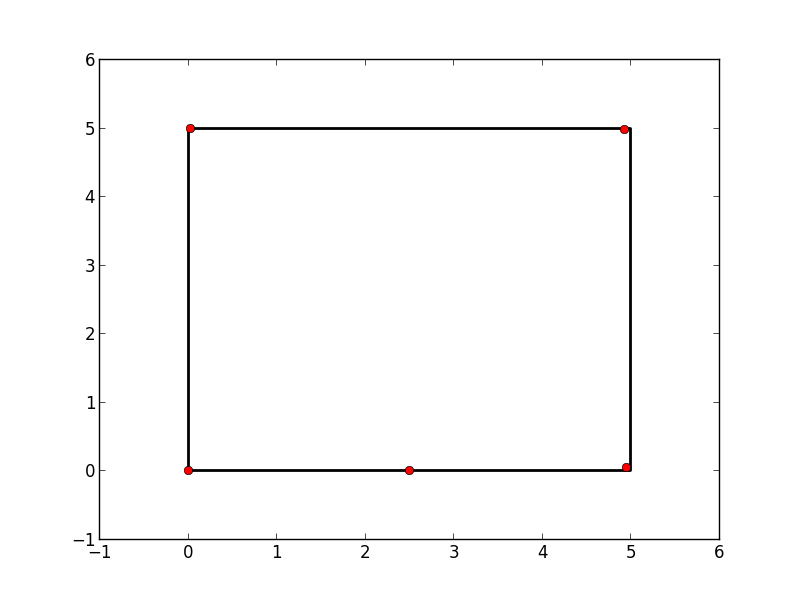
\includegraphics[width=0.7\textwidth]{oplossing_5_vierhoek}
\caption{Resultaat voor het commando \texttt{maxdist 5 vierhoek.txt} met de vierhoek uit de opgave. Dit resultaat werd bekomen na 805 iteraties. De fitnesswaarde bedraagt 44,073322.}
\label{fig:solution_5_vierhoek}
\end{figure}

\begin{figure}[H]
\centering
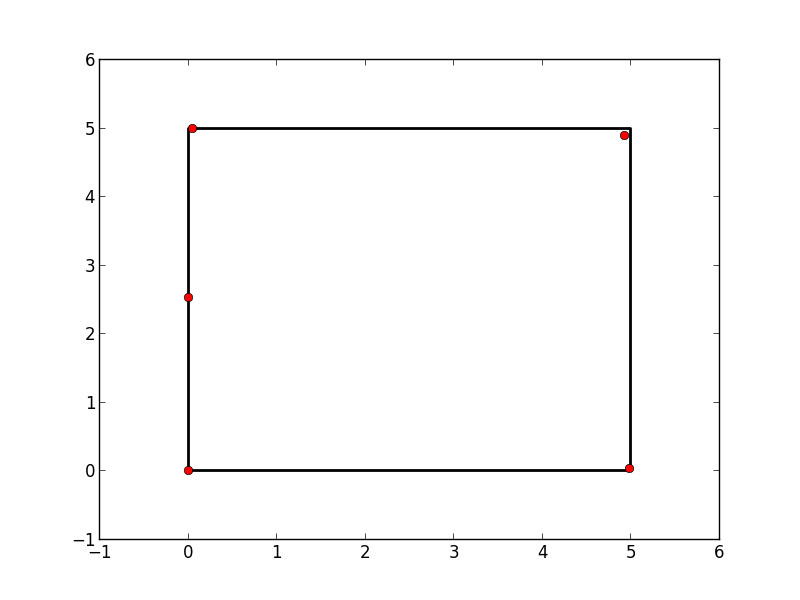
\includegraphics[width=0.7\textwidth]{oplossing_5_vierhoek_uniform_breed}
\caption{Resultaat voor het commando \texttt{maxdist 5 vierhoek.txt} met de vierhoek uit de opgave. Hier werd stochastische bemonstering toegepast om ouders te selecteren en batch selectie om organismen te doden. De fitnesswaarde bedraagt 44,019958. Deze oplossing is bijna even goed als de oplossing in Figuur \ref{fig:solution_5_vierhoek}.}
\label{fig:solution_5_vierhoek_uniform_breed}
\end{figure}

\begin{figure}[H]
\centering
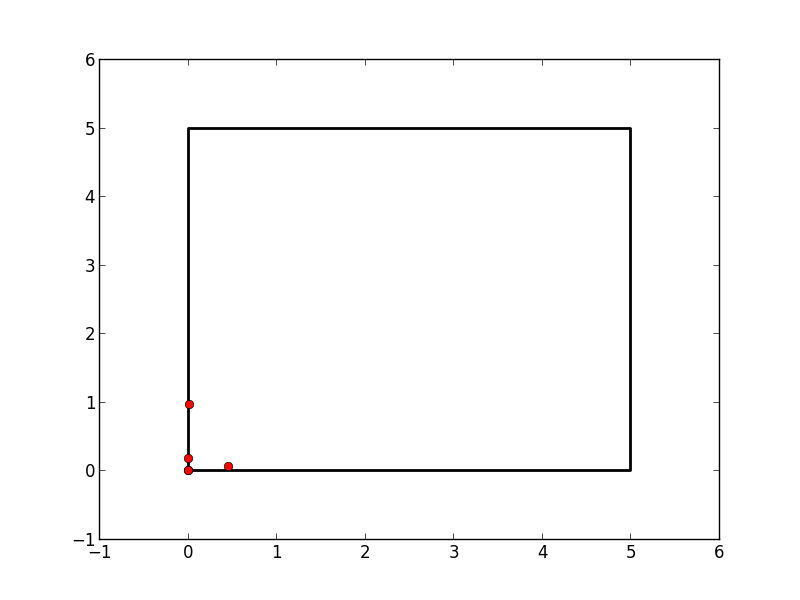
\includegraphics[width=0.7\textwidth]{oplossing_5_vierhoek_both}
\caption{Resultaat voor het commando \texttt{maxdist 5 vierhoek.txt} met de vierhoek uit de opgave. Hier werd stochastische bemonstering toegepast in beide selectiestappen. De fitnesswaarde bedraagt 13,500294. Deze oplossing is duidelijk slecht.}
\label{fig:solution_5_vierhoek_uniform_both}
\end{figure}

\begin{figure}[H]
\centering
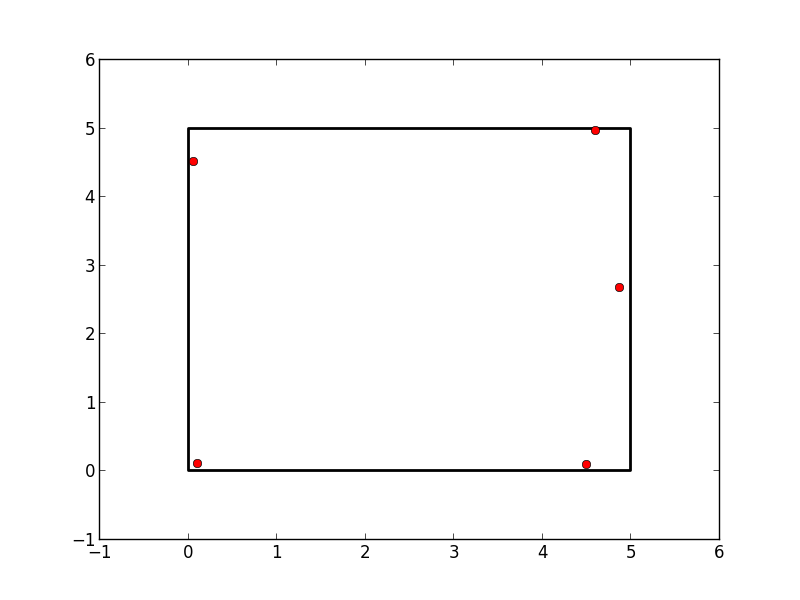
\includegraphics[width=0.7\textwidth]{oplossing_5_vierhoek_death}
\caption{Resultaat voor het commando \texttt{maxdist 5 vierhoek.txt} met de vierhoek uit de opgave. Hier werd stochastische bemonstering toegepast om organismen te doden en batch selectie om ouders te selecteren. De fitnesswaarde bedraagt 42,678516. Ook deze oplossing laat te wensen over.}
\label{fig:solution_5_vierhoek_uniform_death}
\end{figure}

\end{appendices}

\end{document}
